\documentclass[
  captions=tableheading,
  bibliography=totoc, 
  titepage=firstiscover,
]{scrartcl}

\usepackage{blindtext} %neuer input

\usepackage{longtable} % Tabellen über mehrere Seiten

\usepackage[utf8]{inputenc} %neuer input

\usepackage{scrhack}

\usepackage[aux]{rerunfilecheck} %Warnung falls nochmal kompiliert werden muss

\usepackage{fontspec} %Fonteinstellungen

\recalctypearea{}

\usepackage[main=ngerman]{babel} %deutsche Spracheinstellung

\usepackage{ragged2e} %neuer input

\usepackage{amsmath, nccmath}

\usepackage{amssymb} %viele mathe Symbole

\usepackage{mathtools} %Erweiterungen für amsmath


\DeclarePairedDelimiter{\abs}{\lvert}{\rvert}
\DeclarePairedDelimiter{\norm}{\lVert}{\rVert}

\DeclarePairedDelimiter{\bra}{\langle}{\rvert}
\DeclarePairedDelimiter{\ket}{\lvert}{\rangle}

\DeclarePairedDelimiterX{\braket}[2]{\langle}{\rangle}{
#1 \delimsize| #2
}

\NewDocumentCommand \dif {m}
{
\mathinner{\symup{d} #1}
}


\usepackage[
  math-style=ISO,
  bold-style=ISO,
  sans-style=italic,
  nabla=upright,
  partial=upright,
  warnings-off={
    mathtools-colon,
    mathtools-overbracket,
  },
]{unicode-math}

\setmathfont{Latin Modern Math}
\setmathfont{XITS Math}[range={scr, bfscr}]
\setmathfont{XITS Math}[range={cal, bfcal}, StylisticSet=1]


\usepackage[
  locale=DE,
  separate-uncertainty=true,
  per-mode=reciprocal,
  output-decimal-marker={,},
]{siunitx}

\usepackage[autostyle]{csquotes} %richtige Anführungszeichen

\usepackage{xfrac}

\usepackage{float}

\floatplacement{figure}{htbp}

\floatplacement{table}{htbp}

\usepackage[ %floats innerhalb einer section halten
  section,   %floats innerhalb er section halten
  below,     %unterhalb der Section aber auf der selben Seite ist ok
]{placeins}

\usepackage[
  labelfont=bf,
  font=small,
  width=0.9\textwidth,
]{caption}

\usepackage{subcaption} %subfigure, subtable, subref

\usepackage{graphicx}

\usepackage{grffile}

\usepackage{booktabs}

\usepackage{microtype} %Verbesserungen am Schriftbild

\usepackage[
backend=biber,
]{biblatex}

\addbibresource{../lit.bib}

\usepackage[ %Hyperlinks im Dokument
  german,
  unicode,
  pdfusetitle,
  pdfcreator={},
  pdfproducer={},
]{hyperref}

\usepackage{bookmark}

\usepackage[shortcuts]{extdash}

%\usepackage{warpcol}


\begin{document}
    \title{ATP Übungsblatt 7}
    \author{  
    Tobias Rücker\\
    \texorpdfstring{\href{mailto:tobias.ruecker@tu-dortmund.de}{tobias.ruecker@tu-dortmund.de}
    \and}{,} 
    Paul Störbrock\\
    \texorpdfstring{\href{mailto:paul.stoerbrock@tu-dortmund.de}{paul.stoerbrock@tu-dortmund.de}}{}
    }
\maketitle
\center{\Large Abgabegruppe: \textbf{Mittw. 10-12 Uhr}}
\thispagestyle{empty}

\newpage
\tableofcontents
\thispagestyle{empty}
\newpage

\setcounter{page}{1}


\section{Aufgabe 19}

    \begin{figure}[H]
        \centering
        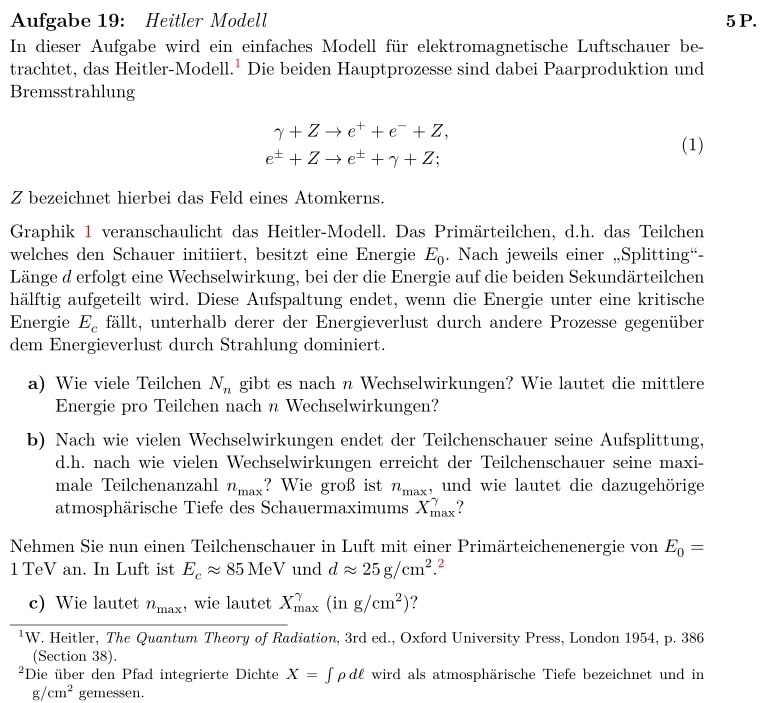
\includegraphics[width=\textwidth]{images/Aufgabe19a.jpg}
        \label{fig:1}
    \end{figure}

    \begin{figure}[H]
        \centering
        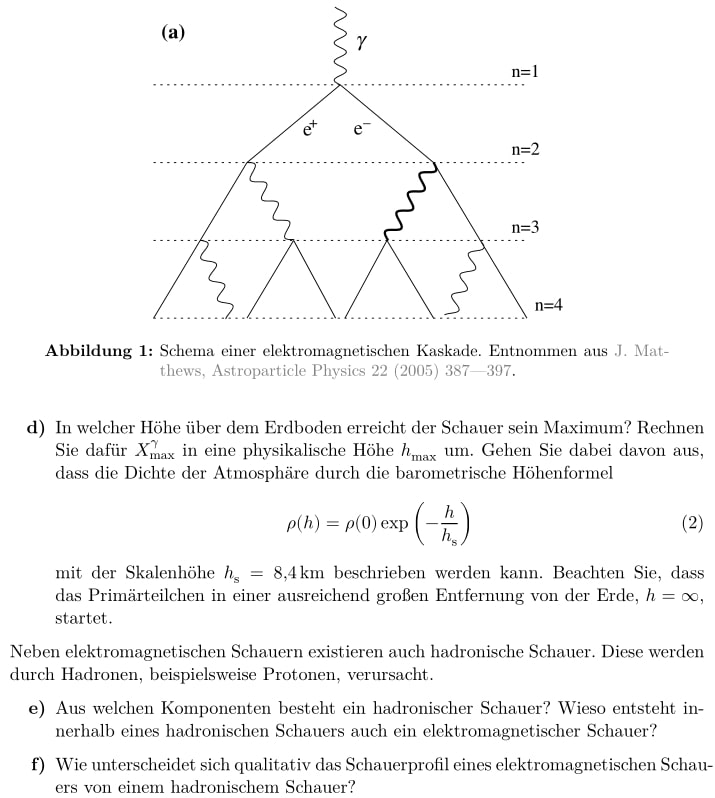
\includegraphics[width=\textwidth]{images/Aufgabe19b.jpg}
        \label{fig:2}
    \end{figure}

\subsection{a)}

\begin{table}[H]
\centering
    \begin{tabular}{c c c c}
    \toprule
    \multicolumn{1}{c}{} & \multicolumn{1}{c}{} & \multicolumn{1}{c}{} & \multicolumn{1}{c}{Teilchenzahl $N_n=n^2$}\\
    \cmidrule(lr{0,5em}){1-4}
    n=0 & p=1 & T=0 & 1\\        
    n=1 & p=0 & T=2 & 2\\       
    n=2 & p=2 & T=2 & 4\\
    n=3 & p=2 & T=6 & 8\\
    n=4 & p=6 & T=10 & 16\\
    n=5 & p=10 & T=22 & 32\\        
    n=6 & p=22 & T=42 & 64\\
    \bottomrule
    \end{tabular}
\label{tab:1}
\end{table}

    \flushleft{Die\;}\justifying mittlere Energie $E_n$ pro Teilchen nach $n$ Wechselwirkungen lautet:
    \begin{align*}
        E_n &= \frac{E_0}{N_n} = \frac{E_0}{n^2}
    \end{align*}

\subsection{b)}

    \flushleft{Ein\;}\justifying Teilchenschauer endet, sobald die Energie jedes Teilchens unter die kritische Energie $E_c$ fällt. Es gilt also:
    \begin{align*}
        E_0 &= N_{n,max} \cdot E_c\\
        \Leftrightarrow E_0 &= 2^{n,max} \cdot E_c\\
        2^{n,max} &= \frac{E_0}{E_c}\\
        \Leftrightarrow n_{max} &= \log_2\left( \frac{E_0}{E_c} \right)
        \intertext{
            \flushleft{Die\;}\justifying atmosphärische Tiefe $X_{max}^{\gamma}$ ergibt sich aus:
        } 
        X_{max}^{\gamma} &= n_{max} \cdot d\\
        &= \log_2\left( \frac{E_0}{E_c} \right) \cdot d
        \intertext{
            \flushleft{Wobei\;}\justifying $d$ die atmosphärische Tiefe eines Splits bezeichnet.
        }
    \end{align*}

\subsection{c)}

    \flushleft{Nach\;}\justifying einsetzten für $E_0$ und $E_c$ ergibt sich für $n_{max}$:
    \begin{align*}
        n_{max} &= \log_2\left( \frac{E_0}{E_c} \right) = 13.52
        \intertext{
            \flushleft{Da\;}\justifying $n \in \mathbb{Z}$, wird hier abgerundet. Daraus folgt:
        }
        n_{max} &= 13\\
        \Rightarrow  X_{max}^{\gamma} &= n_{max} \cdot d = \SI{325}{\gram\per\meter\squared} 
    \end{align*}

\subsection{d)}

    \begin{align*}
        \rho(h) &= \rho(0) exp\left( -\frac{h}{h_s} \right)\\
        X(h) &= \int \rho(h) \mathrm{d}h\\
        X(h_{max}) &= \int_{h_{max}}^{\infty} \rho(0) exp\left( -\frac{h}{h_s} \right) \mathrm{d}h\\
        &= \left[  -\rho(0) h_s exp\left( -\frac{h}{h_s} \right) \right]_{h_{max}}^{\infty}\\
        &= \rho(0) h_s exp\left( -\frac{h_{max}}{h_s} \right) -0\\
        X_{max}^{\gamma} &= \rho(0) h_s exp\left( -\frac{h_{max}}{h_s} \right)\\
        \Leftrightarrow \frac{X_{max}^{\gamma}}{\rho(0) h_s} &= exp\left( -\frac{h_{max}}{h_s} \right)\\
        \Leftrightarrow ln\left( \frac{X_{max}^{\gamma}}{\rho(0) h_s} \right) &= -\frac{h_{max}}{h_s}\\
        \Leftrightarrow h_{max} &= -h_s \cdot ln\left( \frac{X_{max}^{\gamma}}{\rho(0) h_s} \right) = 9197.208
    \end{align*}

\subsection{e)}

    \flushleft{Ein\;}\justifying hadronischer Schauer besteht aus drei Komponenten, der mysonischen Komponente, der hadronischen Komponente und der elektromagnetischen Komponente. 
    Durch die Wechselwirkung zwischen Primärteilchen und der Luft entstehen Teilchen, die den drei Komponenten untergeordnet werden können.\\
    Bei der mysonischen Komponente werden Kaonen (+,-,0) und Pionen (+,-) erzeugt, die anschließend zu Myonen und Neutrinos zerfallen.\\
    Bei der hadronischen Komponente wird eine hadronische Kaskade erzeugt, die sich aus Protonen, Neutronen, Pionen (+,-) und Kaonen (+,-) zusammensetzt.\\
    Bei der elektromagnetischen Komponente werden Kaonen (+,-,0) und Pionen (+,-,0) erzeugt. Pionen (+,-) und Kaonen (+,-,0) zerfallen schließend zu Myonen (+,-), welche dann 
    zu Elektronen $e^-$ und Positronen $e^+$ zerfallen. Diese emittieren durch Energieverlust Bremsstrahlung (Cherenkovstrahlung und Fluoreszenzstrahlung). Das neutrale Pion 
    zerfällt zu zwei $\gamma$-Photonen. Diese Photonen besitzen hingegen genug Energie um durch Paarproduktion auch jeweils ein $e^+$ und $e^-$ zu erzeugen, welche wiederum
    anschließend Cherenkov-/Fluoreszenzstrahlung erzeugen. 

    \flushleft{Der\;}\justifying EM-Schauer ensteht durch den Zerfall in $e^+$ und $e^-$, welche die EM-Komponente ausmachen. 
    

\subsection{f)}

    \flushleft{Ein\;}\justifying EM-Schauer erzeugt bei Detektion einen relativ einheitlichen und engen Lichtkegel an Cherenkovlicht.\\
    Ein hadronischer Schauer hingegen ist breiter gestreut. Der footprint eines hadronischen Schauers setzt sich aus mehreren kleinen Kegelprofilen (Hotspots) zusammen.  


\section{Aufgabe 20}

    \begin{figure}[H]
        \centering
        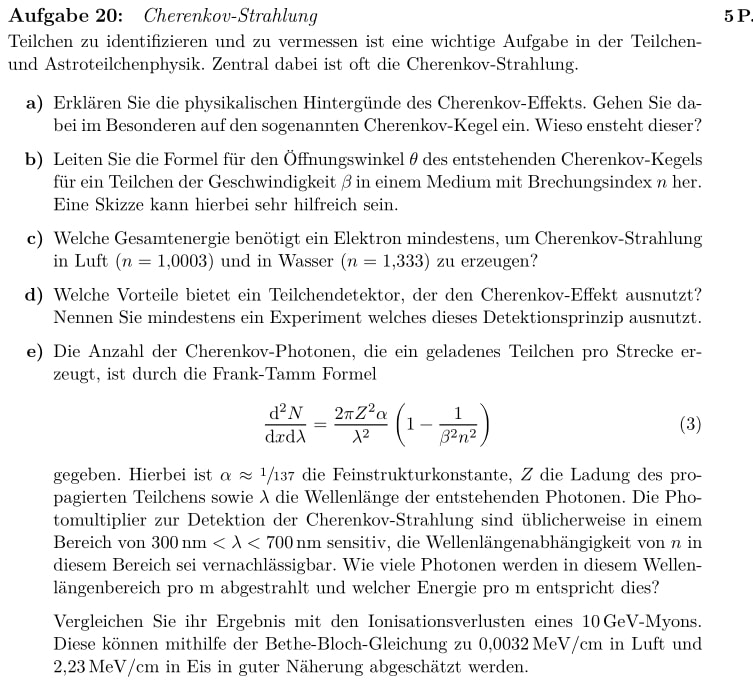
\includegraphics[width=\textwidth]{images/Aufgabe20.jpg}
        \label{fig:3}
    \end{figure}


\subsection{a)}
Beim Cerenkov-Effekt bewegt sich ein Teilchen in einem Medium mit Brechungsindex n schneller als das Licht in diesem Medium.
Die durch das Teilchen erzeugten Kugelwellen entlang der Trajektorie überlagern sich, sodass eine Kegelförmige Wellenfront
entsteht.
\begin{figure}
    \centering
    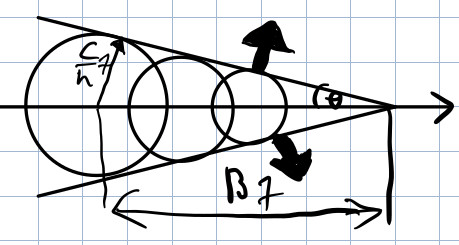
\includegraphics[width=0.5\textwidth]{images/kegel.jpg}
\end{figure}

\subsection{b)}
\begin{figure}
\centering
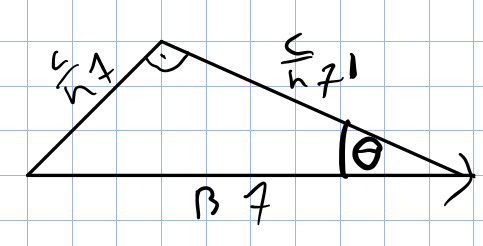
\includegraphics[width=0.5\textwidth]{images/winkel.jpg}
\end{figure}
\begin{align}
\theta = \arcsin \left( \frac{c}{n \beta} \right)
\end{align}
\subsection{c)}
\begin{align}
\beta &= \frac{c}{n}\\
E&= \gamma m_0 c^2\\
&= \frac{m_e c^2}{\sqrt{1-\frac{\beta ^2}{c^2}}}\\
&= \frac{m_e c^2}{\sqrt{1-\frac{1}{n^2}}}\\
\intertext{
    Für Luft
}
E = \input{luft.tex}
\intertext{
    Für Wasser
}
E =\input{wasser.tex}
\end{align}

\subsection{d)}
Die Vorteile eines Teilchendetektors, der den Cherenkov-Effekt ausnutzt ist der, dass
zum einen das dieser sensitiv für die Einfallrichtung ist. Das heißt man kann
bestimmen aus welcher Richtung Leptonen-Schauer kommen und damit Quellen dieser finden.
Zudem müssen die Signale nicht im Detektor landen, da diese Kegel ein ganzes Stück bewegen können. 
Dadurch ist der messbare Bereich ein ganzes Stück größer als der eigentliche Detektor.
Ein Beispiel bildet der Ice-Cube-Detektor am Südpol.

\subsection{e)}
Unter Vernachlässigung von n für ein Photon
\begin{align}
    \frac{\dif{N}}{\dif{x}} &= \int_{300nm}^{700nm} \frac{2 \pi \alpha}{\lambda^2} \,\dif{\lambda}\\
    &= (-\frac{1}{700nm}+\frac{1}{300nm}) 2 \pi \alpha \\
    \approx 87.357 Photonen/m
    E&=\frac{hc}{\lambda}
    \frac{E}{l} &= \int_{300nm}^{700nm} h \frac{c}{\lambda} \,\dif{\lambda}\\
    &= ch(\ln (700nm)-\ln(300nm) )\\
    \intertext{
        N für 1m
    }
    \frac{E}{l} &= N_{1m} ch \ln \left(\frac{7}{3} \right)\\
    &= \SI{0.09}{\electronvolt\per\meter}\\
    &= \SI{90}{\milli\electronvolt\per\centi\meter}
\end{align}
Die berechnete Energie ist wesentlich kleiner als die Energie des \SI{10}{\giga\electronvolt}-Myons.


\section{Aufgabe 21}

    \begin{figure}[H]
        \centering
        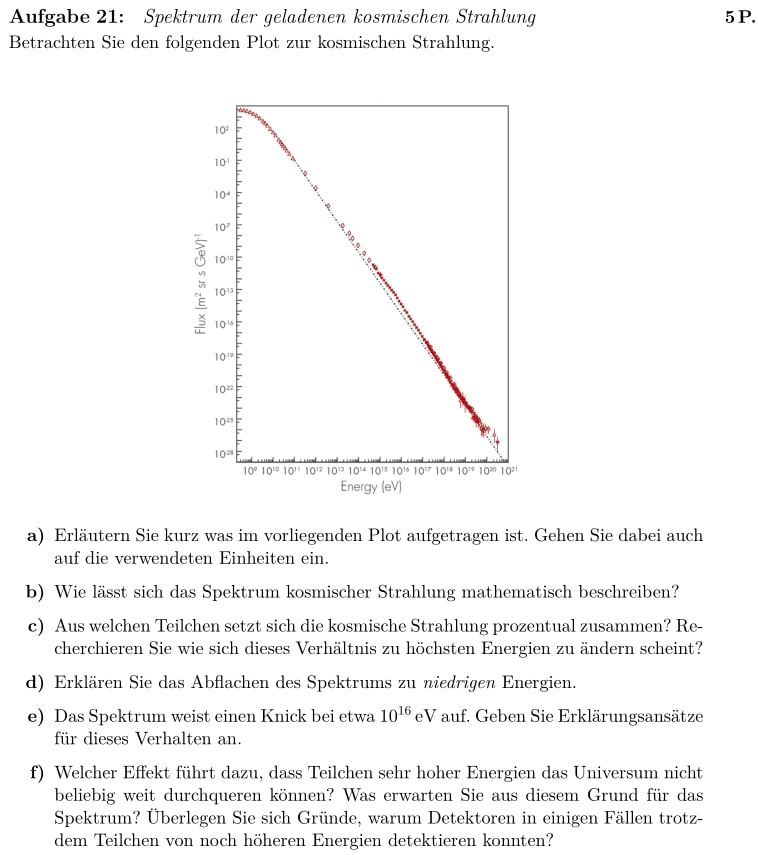
\includegraphics[width=\textwidth]{images/Aufgabe21.jpg}
        \label{fig:4}
    \end{figure}


\subsection{a)}

    \flushleft{Das\;}\justifying in Audgabe 21 abgebildete Diagramm beschreibt die Energie der geladenen kosmischen Strahlung (Cosmic Rays), die über eine Fläche pro Zeiteinheit (Flux)
    gemessen werden. Deutlich zu erkennen sind die zwei Anhäufungen an Messwerten oben links und mitte- bis unten rechts. Der Teil der Messwerte zwischen $10^{8}$ \SI{}{\giga\electronvolt}
    und $10^{17}$ \SI{}{\giga\electronvolt} ist der nicht-relativistische Teil der Strahlung und der von $10^{17}$ \SI{}{\giga\electronvolt} fortlaufende Teil ist relativistisch.\\
    Besonders auffällig sind zwei Bereiche im Graphen, die als Knie und Ferse (knee and heel) beschrieben werden. Das Knie liegt im Bereich von $10^{15}$ \SI{}{\giga\electronvolt}
    bis $10^{16}$ \SI{}{\giga\electronvolt} und die Ferse im Bereich von $10^{18}$ \SI{}{\giga\electronvolt} bis $10^{19}$ \SI{}{\giga\electronvolt}.

\subsection{b)}

    \flushleft{Mit\;}\justifying dem Potentialansatz $N=E^{-\gamma}$ lässt sich der Flux energieabhängig darstellen. Der Exponen $\gamma$ ist relativ gleichbleibend, da im Diagramm
    eine klarer exponentieller Abfall erkennbar ist. An den in a) beschrieben Stellen (Knie und Ferse) verändert sich dieser Wert hingegen stärker.

\subsection{c)}

    \flushleft{Die\;}\justifying Cosmic Rays, die auf der Erde gemessen werden bestehen zum Großteil (ca. 89\%) aus Protonen, dem Kern eines Wasserstoffatoms. 10\% der Strahlung 
    besteht aus Heliumnuclei und der letzte Prozent setzt sich aus schwereren Nuclei zusammen. 
    Bei höheren Energien tendiert dieses Verhältniss hingegen zu schwereren Teilchen. Diese besitzten zum Teil ausreichend Energie, um aus einer anderen Energie zu entkommen. Demnach 
    kann ein hochenergetisches Teilchen enorme Distanzen zurücklegen. Jedoch ist die Wahrscheinlichkeit, ein solches Teilchen zu messen dementsprechend gering. 

\subsection{d)}

    \flushleft{Niederenergetische\;}\justifying Teilchen haben zu wenig Energie um das Magnetfeld der Erde zu durchbrechen. Niederenergetische Strahlung, die von der Sonne emittiert 
    wird, kann vom Erdmagnetfeld abgeschrirmt werden. Teilchen oder Strahlung, die von außerhalb unseres Sonnensystems stammt, muss zudem das Magnetfeld der Sonne durchqueren. 

\subsection{e)}

    \flushleft{Das\;}\justifying Knie, welches bei ca. $10^{16}$ \SI{}{\giga\electronvolt} liegt, stellt einen nicht-exponentiell abfallenden Flux bei steigender Energie dar. Also, dass 
    sich die Zählrate der Teilchen bei steigender Teilchenenergie ähnelt. Es staut sich demnach ein bestimmter Teil an Teilchen in diesem Energiebereich auf. Eine mögliche Erklärung
    wäre binäre Neutronensternsysteme, die hochenergetische Strahlung emittieren. Außerdem befindet sich da Knie am unteren nicht-relativistischen Bereich, weshalb sich der starke
    Abfall unmittelbar nach dem Knie auf die hohe Geschwindigkeit des Teilchens zurückführen lassen könnte. Das Magnetfeld der Sonne kann auch hier einen Teil der niederenergetischen
    Strahlung ablenken, sodass uns diese Teilchen garnicht erreichen. 

\subsection{f)}

    \flushleft{Teilchen\;}\justifying mit Energien höher als $10^{20}$ \SI{}{\giga\electronvolt}, also ultra hochenergetische (UHE) Protonen, haben eine mittlere Weglänge von ca. 100 bis
    150 ly, was bedeutet, dass solche Teilchen innerhalb unserer Milchstraße entstehen sollten. Der Energiebereich oberhalb von $10^{20}$ \SI{}{\giga\electronvolt} wird auch als 
    Greisen-Zatsepin-Kuz'min-cutoff (GZK-cutoff) bezeichnet, da Greisen, Zatsepin und Kuz'min diese Energie erstmals im Jahre 1966 als Grenze der CR annahmen. UHE Protonen haben 
    genug Energie um mit den Photonen der CBR wechselwirken zu können. Dadurch verlieren die Protonen an Energie, wodurch die Grenze bei $10^{20}$ \SI{}{\giga\electronvolt} nicht
    überschritten wird. 


\end{document}